% This is samplepaper.tex, a sample chapter demonstrating the
% LLNCS macro package for Springer Computer Science proceedings;
% Version 2.20 of 2017/10/04
%
\documentclass[runningheads]{llncs}
%
\usepackage{graphicx}
\usepackage{multirow} 
\usepackage{fancyvrb}
\usepackage[misc,geometry]{ifsym} 
\usepackage{subcaption}
\usepackage{caption}
\usepackage{listings}
\usepackage{xcolor}
\usepackage{booktabs}
\newcommand{\ra}[1]{\renewcommand{\arraystretch}{#1}}
\setlength{\tabcolsep}{0.7em}

\lstloadlanguages{Python}
\lstset{
  language=Python,
  basicstyle=\scriptsize\sffamily,
  numberstyle=\color{gray},
  stringstyle=\color[HTML]{933797},
  commentstyle=\color[HTML]{228B22}\sffamily,
  emph={[2]from,import,pass,return}, emphstyle={[2]\color[HTML]{DD52F0}},
  emph={[3]range}, emphstyle={[3]\color[HTML]{D17032}},
  emph={[4]for,in,def}, emphstyle={[4]\color{blue}},
  showstringspaces=false,
  breaklines=true,
  prebreak=\mbox{{\color{gray}\tiny$\searrow$}},
  numbers=left,
  xleftmargin=15pt
}

% Used for displaying a sample figure. If possible, figure files should
% be included in EPS format.
%
% If you use the hyperref package, please uncomment the following line
% to display URLs in blue roman font according to Springer's eBook style:
\usepackage{hyperref}
\renewcommand\UrlFont{\color{blue}\rmfamily}

\begin{document}
%
\title{Genegram: RNA Secondary Structure Prediction Using Formal Grammars and Residual Neural Networks\thanks{Supported by the Russian Science Foundation grant 18-11-00100}}
%
\titlerunning{Genegram: CFG + ResNet}
% If the paper title is too long for the running head, you can set
% an abbreviated paper title here
%
\author{Polina Lunina\inst{1,2}\orcidID{0000-0002-7172-2647} \Letter \and
Semyon Grigorev\inst{1,2}\orcidID{0000-0002-7966-0698} \and
Vadim Abzalov\inst{1,2}\orcidID{0000-0002-0805-0315}}
%
\authorrunning{Polina Lunina, Semyon Grigorev, Vadim Abzalov}
% First names are abbreviated in the running head.
% If there are more than two authors, 'et al.' is used.
%
\institute{Saint Petersburg State University, 7/9 Universitetskaya nab., St. Petersburg, 199034, Russia \and
JetBrains Research, Primorskiy prospekt 68-70, Building 1, St. Petersburg 197374, Russia\\
\email{lunina\_polina@mail.ru \Letter, semyon.grigorev@jetbrains.com, vadim.i.abzalov@gmail.com}\\
}
%
\maketitle             % typeset the header of the contribution
%
\begin{abstract}
Improvement in RNA secondary structure prediction accuracy is one of the key focuses in computational genomics due to its crucial role in the functional analysis of RNA molecules. We propose a new approach to solve this problem. Simple context-free grammar describes the most common types of stems and the parsing matrix for some sequence represents all the theoretically possible folds for each subsequence. This information is excessive because only one combination of stems will be presented in a real secondary structure. Moreover, the parsing matrix can be incomplete due to inevitable limitations in grammar. So, we process parsing matrices with residual neural networks in order to generate a valid secondary structure. This approach allows to process pseudoknots, wobble base pairs, and multiple contacts due to the flexible nature of the neural network training process. Our solution was implemented as a Python console tool Genegram.

\keywords{RNA \and Secondary Structure \and Genomic Sequences \and CNN \and ResNet \and Machine Learning  \and Formal Grammars \and Parsing.}
\end{abstract}
%
%
%
\section{Introduction}
\section{Introduction}

Scalable high-performance graph analysis is an actual challenge.
There is a big number of ways to attack this challenge~\cite{Coimbra2021} and the first promising idea is to utilize general-purpose graphic processing units (GPGPU-s).
Such existing solutions, as CuSha~\cite{10.1145/2600212.2600227} and Gunrock~\cite{7967137} show that utilization of GPUs can improve the performance of graph analysis, moreover it is shown that solutions may be scaled to multi-GPU systems.
But low flexibility and high complexity of API are problems of these solutions.

The second promising thing which provides a user-friendly API for high-performance graph analysis algorithms creation is a GraphBLAS API~\cite{7761646} which provides linear algebra based building blocks to create graph analysis algorithms.
The idea of GraphBLAS is based on is a well-known fact that linear algebra operations can be efficiently implemented on parallel hardware.
Along with this, a graph can be natively represented using matrices: adjacency matrix, incidence matrix, etc.
While reference CPU-based implementation of GraphBLAS, SuiteSparse:GraphBLAS~\cite{10.1145/3322125}, demonstrates good performance in real-world tasks, GPU-based implementation is challenging.

One of the challenges in this way is that real data are often sparse, thus underlying matrices and vectors are also sparse, and, as a result, classical dense data structures and respective algorithms are inefficient. 
So, it is necessary to use advanced data structures and procedures to implement sparse linear algebra, but the efficient implementation of them on GPU is hard due to the irregularity of workload and data access patterns.
Though such well-known libraries as cuSparse show that sparse linear algebra operations can be efficiently implemented for GPGPU-s, it is not so trivial to implement GraphBLAS on GPGPU. 
First of all, it requires \textit{generic} sparse linear algebra, thus it is impossible just to reuse existing libraries which are almost all specified for operations over floats.
The second problem is specific optimizations, such as maskings fusion, which can not be natively implemented on top of existing kernels.
Nevertheless, there is a number of implementations of GraphBLAS on GPGPU, such as GraphBLAST:~\cite{yang2019graphblast}, GBTL~\cite{7529957}, which show that GPGPUs utilization can improve the performance of GraphBLAS-based graph analysis solutions.
But these solutions are not portable because they are based on Nvidia Cuda stack.
Moreover, the scalability problem is not solved: all these solutions support only single-GPU, not multi-GPU computations.

To provide portable GPU implementation of GraphBLAS API we developed a \textit{SPLA} library (sources are published on GitHub: \url{https://github.com/JetBrains-Research/spla}).
This library utilizes OpenCL for GPGPU computing to be portable across devices of different vendors.
Moreover, it is initially designed to utilize multiple GPGPUs to be scalable.
To sum up, the contribution of this work is the following.
\begin{itemize}
    \item Design of portable GPU GraphBLAS implementation proposed. The design involves the utilization of multipole GPUS. Additionally, the proposed design is aimed to simplify library tuning and wrappers for different high-level platforms and languages creation. 
    \item Subset of GraphBLAS API, including such operations as masking, matrix-matrix multiplication, matrix-matrix e-wise addition, is implemented. The current implementation is limited by COO and CSR matrix representation format and uses basic algorithms for some operations, but work in progress and more data formats will be supported and advanced algorithms will be implemented in the future.
    \item Preliminary evaluation on such algorithms as breadth-first search (BFS) and triangles counting (TC), and real-world graphs shows portability across different vendors and promising performance: for some problems Spla is comparable with GraphBLAST. Surprisingly, for some problems, the proposed solution on embedded Intel graphic card shows better performance than SuiteSparse:GraphBLAS on the same CPU. At the same time, the evaluation shows that further optimization is required.
\end{itemize} 

\section{Proposed Approach Overview}
In this section, we focus more on the theoretical aspects of the proposed approach that underlie the experimental research presented in section 3. 

Secondary structure can be viewed as a recursive composition of stems having different lengths and loop sizes~\cite{MQbioinformatics19}, so, we propose to use formal grammar to encode the most common types of stems, considering RNA sequence as a string in the $\{A, C, G, U\}$ alphabet. Thereby, the parsing matrix for some sequence will contain information about whether each subsequence of this sequence can fold to stem or not. This matrix is not yet a representation of a valid secondary structure, because all these stems cannot exist at once and, besides, there can be more complex elements that are not expressible in terms of given grammar (for example, pseudoknots and wobble base pairs). Therefore, we propose to process parsing matrices by neural networks that should filter extra stems and add the missing elements in order to generate a maximal approximation of real secondary structure in some compatible with another studies format. In figure~\ref{arch} the global solution architecture is presented and in the next sections, we will speak in detail about each of the specified components.

\begin{figure}[h]
\centering
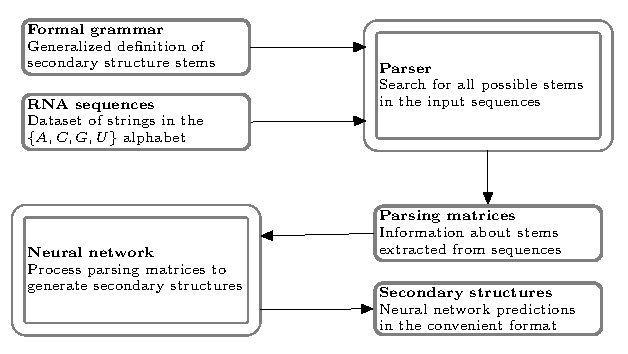
\includegraphics[width=\textwidth]{pics/arch.pdf}
\caption{Global solution architecture}
\label{arch}
\end{figure}

\subsection{Formal Grammar}
As it was mentioned before, our approach employs formal grammar not for modeling the whole structure, but for encoding its simple constructional elements (stems), therefore this grammar does not require probabilistic rules --- probability estimation is to be done by neural networks. We do not strictly fix the grammar and it can be modified in accordance with research purposes or data characteristics, so, the grammar presented below is just a concrete example that showed quite successful results during the experiments.

In figure~\ref{gram} context-free grammar $G_0$ that we use in this work as well as in the previous ones is presented. This grammar describes the recursive compositions of stems having height at least 3 (lines \textbf{7-12}) and loop size from 1 up to 20 (line \textbf{3}). Note that these constants are not mandatory and might be defined experimentally for each task. Also, $G_0$ allows only four classical nucleotides (line \textbf{4}) and conventional base pairs (line \textbf{5}), because adding the rules for more pairs and nucleotides complicates the grammar unacceptably in the context of performance, moreover, context-free grammars cannot explicitly express pseudoknots, therefore, we expect the neural network to handle all these features instead. Also, we consider only stems of height three or more (lines \textbf{1-2}), because including shorter stems would overload the parsing matrix with too much extra information. So, by this rules, a sequence folds to stem if and only if it is derivable from start nonterminal $start$ of $G_0$ (line \textbf{1}).

\begin{figure}[ht]
\begin{Verbatim}[numbers=left,xleftmargin=5mm]
start: stem3<s0>
s0: loop | loop stem3<s0> s0
loop: nucl*[1..20]
nucl: A | U | C | G
stem1<s>: A s U | G s C | U s A | C s G
stem2<s>: stem1<stem1<s>>
stem3<s>: 
      stem1<stem2<s>>
    | A stem3<s> U
    | U stem3<s> A
    | C stem3<s> G
    | G stem3<s> C
\end{Verbatim}
\caption{Context-free grammar $G_0$ for RNA secondary structure stems description}
\label{gram}
\end{figure}

Having a grammar, we want to find all the subsequences of some given sequence that may fold to stems and this is to be done by means of parsing. Formally, the result of a matrix-based parsing algorithm for an input string $w$ is an upper-triangular boolean matrix $M_P$, where $M_P [i,j] = 1$ if and only if the substring $w[i,j]$ is derivable from grammar start nonterminal. From the practical point of view, this means that parsing matrix contains one in a cell if and only if a correspondent substring folds to stem according to the rules of a given grammar, so, each stem results in a diagonal chain of ones in the matrix, because if sequence $w_1...w_n$ is a stem than it is clear that $w_2...w_{n - 1}$ is a stem, $w_3...w_{n - 2}$ is a stem and so on while the stem height is at least 3.

In figure~\ref{pars_res} we provide the parsing result for a short RNA sequence and show how parsing matrix maps with secondary structure stems. Each one cell describes the stem of height at least 3, so, this sequence contains two subsequences that may fold to stems of the first nesting level. These stems expected hydrogen bonds along with corresponding matrix cells are painted in two different colors. All nucleotide bonds forming a stem of height three or more are represented by solid lines, moreover, it is obvious that each stem of height three encapsulates stems of heights two and one which are highlighted by dotted lines. Note that these stems interfere with each other, thereby, secondary structure cannot contain both of them at the same time. So, the parsing matrix for a sequence describes all the theoretically possible folds there, but at the current step, we cannot know which one of them would be presented in the real secondary structure. Moreover, $G_0$ has certain limitations, such as stem height, loop size, and possible base pairs, so, some of the required stems may be missing in the parsing matrix. While creating a grammar we were guided by two competing ideas: to cover as many types of stems as possible and to stay with an adequate amount of extra information in the parsing matrix along with acceptable time costs for parsing.

\begin{figure}[h]
\centering
\valign{#\cr
  \hbox{%
    \begin{subfigure}[b]{.6\textwidth}
    \centering
    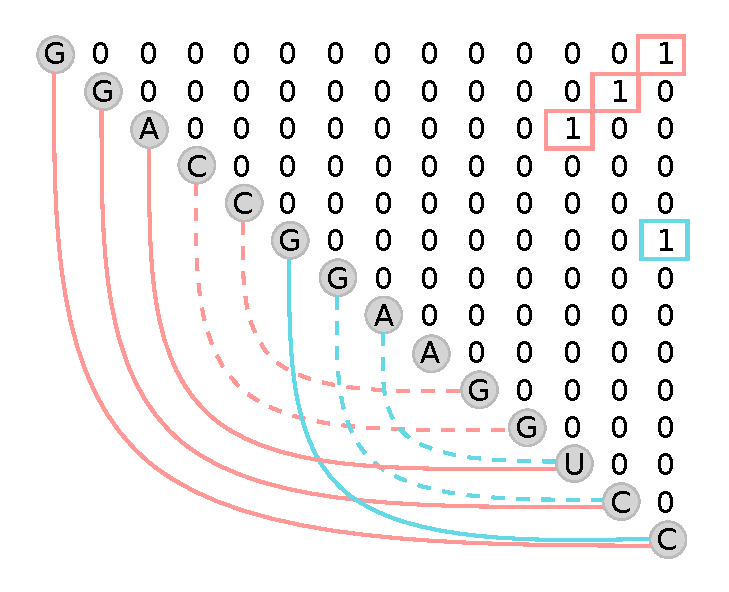
\includegraphics[width=\textwidth]{pics/matrix.pdf}
    \caption{Parsing matrix}
    \label{mtrx}
    \end{subfigure}%
  }\cr
  \noalign{\hfill}
  \hbox{%
    \begin{subfigure}{.4\textwidth}
    \centering
    \vspace{2mm}
    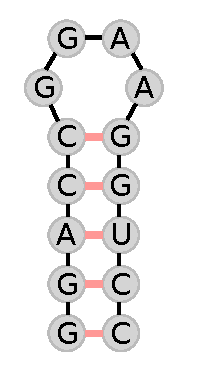
\includegraphics[width=.3\textwidth]{pics/stem1.pdf}
    \caption{First stem}
    \label{stem1}
    \end{subfigure}%
  }\vfill
  \hbox{%
    \begin{subfigure}{.4\textwidth}
    \centering
     \vspace{-2mm}
    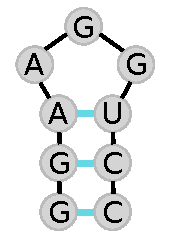
\includegraphics[width=.3\textwidth]{pics/stem2.pdf}
    \caption{Second stem}
    \label{stem2}
    \end{subfigure}%
  }\cr
}
\caption{Stems extracted from RNA sequence by parser}
\label{pars_res}
\end{figure}

Let us consider pseudoknotted structures processing. Even though it is clear that pseudoknot is not explicitly expressed in $G-0$, as well as in any context-free grammar, it consists of two stem-loop structures having half of one stem located between two halves of another, so, each of these stems separately can be derived by the rules of $G_0$. Therefore, pseudoknots will be reflected in the parsing matrix, and handling them becomes an additional task for a neural network. In figure~\ref{pk} an example of simple pseudoknot along with corresponding parsing result is provided. Two stems of this pseudoknot are highlighted with two different colors and it can be seen that all the related nucleotide bonds are presented in the parsing matrix, although at this point it is not determined whether this sequence contains a pseudoknot or it just has two possible folds in terms of grammar.

\begin{figure}[h]
\centering
\begin{subfigure}{.3\textwidth}
  \centering
  \hbox{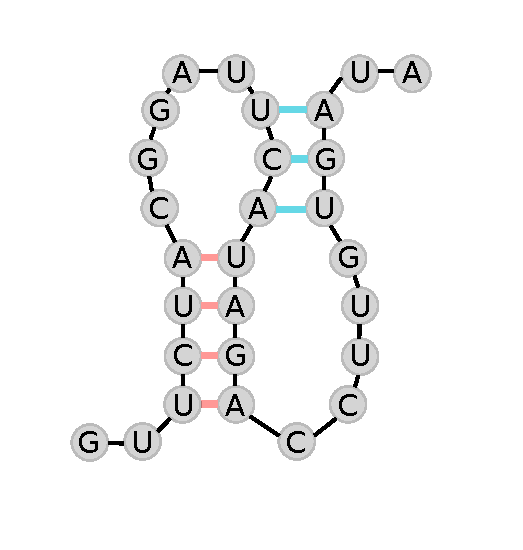
\includegraphics[width=.9\linewidth]{pics/pk.pdf}}
  \caption{Pseudonkot}
  \label{pk_a}
\end{subfigure}%
\begin{subfigure}{.7\textwidth}
  \centering
  \hbox{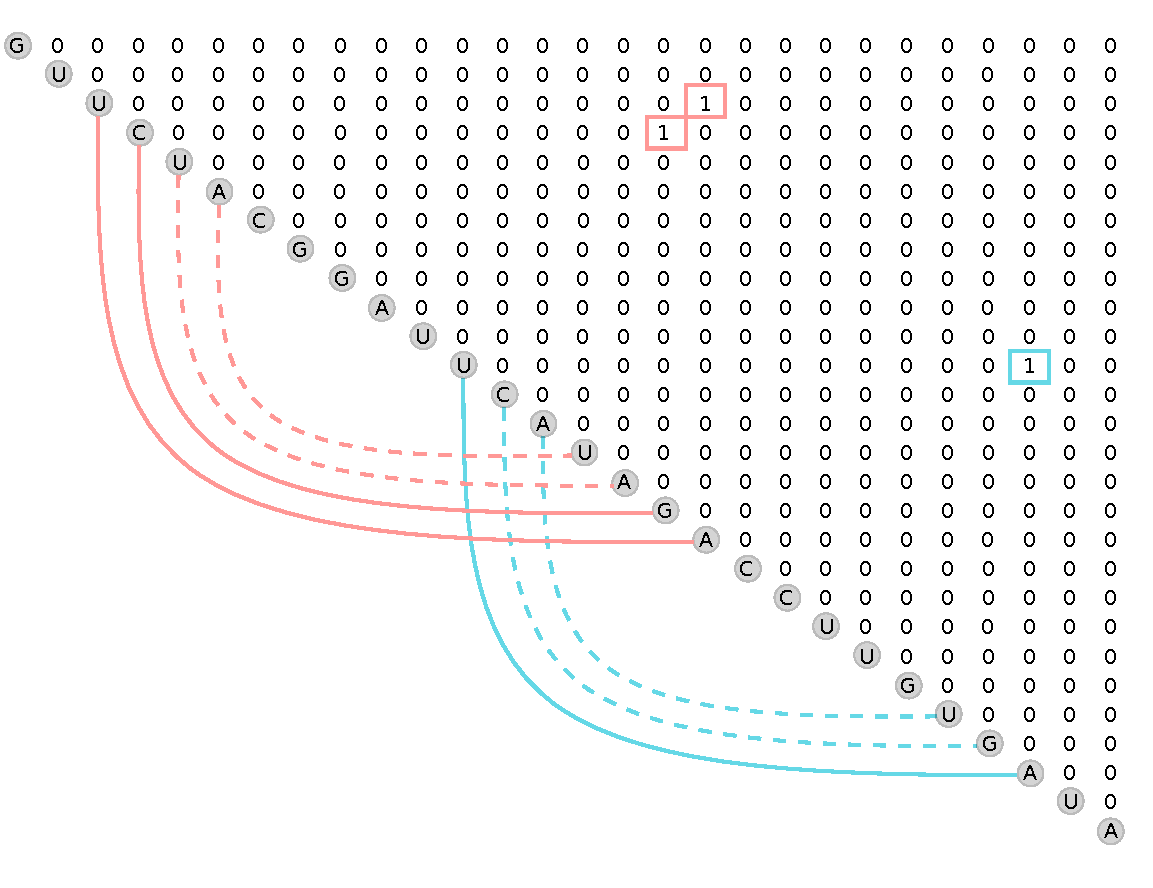
\includegraphics[width=.9\linewidth]{pics/matrix_pk.pdf}}
  \caption{Parsing matrix}
  \label{pk_b}
\end{subfigure}
\caption{Pseudoknots processing in terms of $G_0$}
\label{pk}
\end{figure}

To sum up, our grammar explicitly or implicitly describes a wide range of secondary structure elements and even the missing ones do not become a problem for our approach --- neural network is still capable to handle them. We think of such flexibility as one of the key advantages of our solution.

\subsection{Neural Network}
The matrix that our parser produced for some sequence and fixed grammar should be processed by a neural network in order to achieve a maximal similarity with the expected secondary structure for this sequence. Therefore, we need to specify the data preparing pipeline and describe the required architecture for the problem at hand. It should be noted that these are global and permanent aspects in the context of current work, however, both of them can and probably will be changed while conducting some different research.

\subsubsection{Data}
The input data for neural network (parsing matrices) was described in the previous section and now let us define the reference data source and format. There are specialized biological databases containing RNA chains of various organisms along with their secondary structures obtained by reliable methods, and such data is known to be the best for algorithms training and validation. These databases may store data using different representations (dot-bracket, connectivity table, and others), so, we need to choose a format that is convenient for our experiments and compatible with others.

One of the ways of RNA secondary structure formal representation is so-called contact map, which for an input string $w$ is a boolean matrix $M_C$, where $M_C [i,j] = 1$ if and only if nucleotides in positions $i$ and $j$ form a hydrogen bond (or, to put it simply, a contact) in secondary structure. Even though it is not the most popular format, contact matrix can be easily obtained from the corresponding connectivity table, moreover, there are certain tools that transform connectivity tables to dot-brackets~\cite{bellaousov2013rnastructure}, which provides the required compatibility. Let us consider for the above sequence $w$ the discussed earlier parsing matrix $M_P$ that has $M_P[i, j] = 1$ if and only ifsubsequence $w[i, j]$ folds to a stem. It is clear that the first and the last nucleotides of every stem form a contact, therefore, we can easily transfer between parsing matrix and contact map definitions and view the parsing matrix as a sort of a contact map, so, this format is convenient for our experiments. Note that if parser finds a stem of height three than we will see only one cell with $1$ in matrix, but such stem always wraps a stem of height two which wraps a stem of height one, so, we are always missing two contacts, therefore, after parsing we should set $M_P[i - 1, j + 1] := 1$ , $M_P[i - 2, j + 2] := 1$ if $M_P[i][j] = 1$, $i = 0..size(M_P), j = i + 1..size(M_P)$ for complete semantic equality of parsing and contact matrices.

So, a neural network should take parsing matrices as inputs and contact maps as desired outputs for the same set of RNA sequences. For convenience, we transform both matrices to black-and-white images by replacing zero cells with black pixels and one cells with white pixels. Also, we code RNA sequence at the input image main diagonal by four types of gray pixels corresponding to the four possible nucleotides in case the chain itself contains any important information about secondary structure formation patterns.

In figure~\ref{struc} we provide two-dimensional secondary structure visualization for RNA sequence along with neural network input and reference images that were made from parsing and contact matrices respectively. Contacts belonging to the three stems presented in this sequence are highlighted with three different colors in all pictures (so, input and reference images are actually grayscale, colored pixels are only here for clarification). It can be seen that not all of the stems found by the parser are presented in the real secondary structure. Moreover, the parsing result is missing several contacts since they were formed by non-canonical nucleotide pairs $A-G$ that are not expressed by grammar $G_0$. Now the purpose of a neural network becomes clear --- it should take image~\ref{struc_b} and transform it to the image~\ref{struc_c} as accurately as possible. And the ideas behind this transformation are outlined in the next section.

\captionsetup[subfigure]{justification=centering}
\begin{figure}[h]
\centering
\begin{subfigure}{.33\textwidth}
  \centering
  \hbox{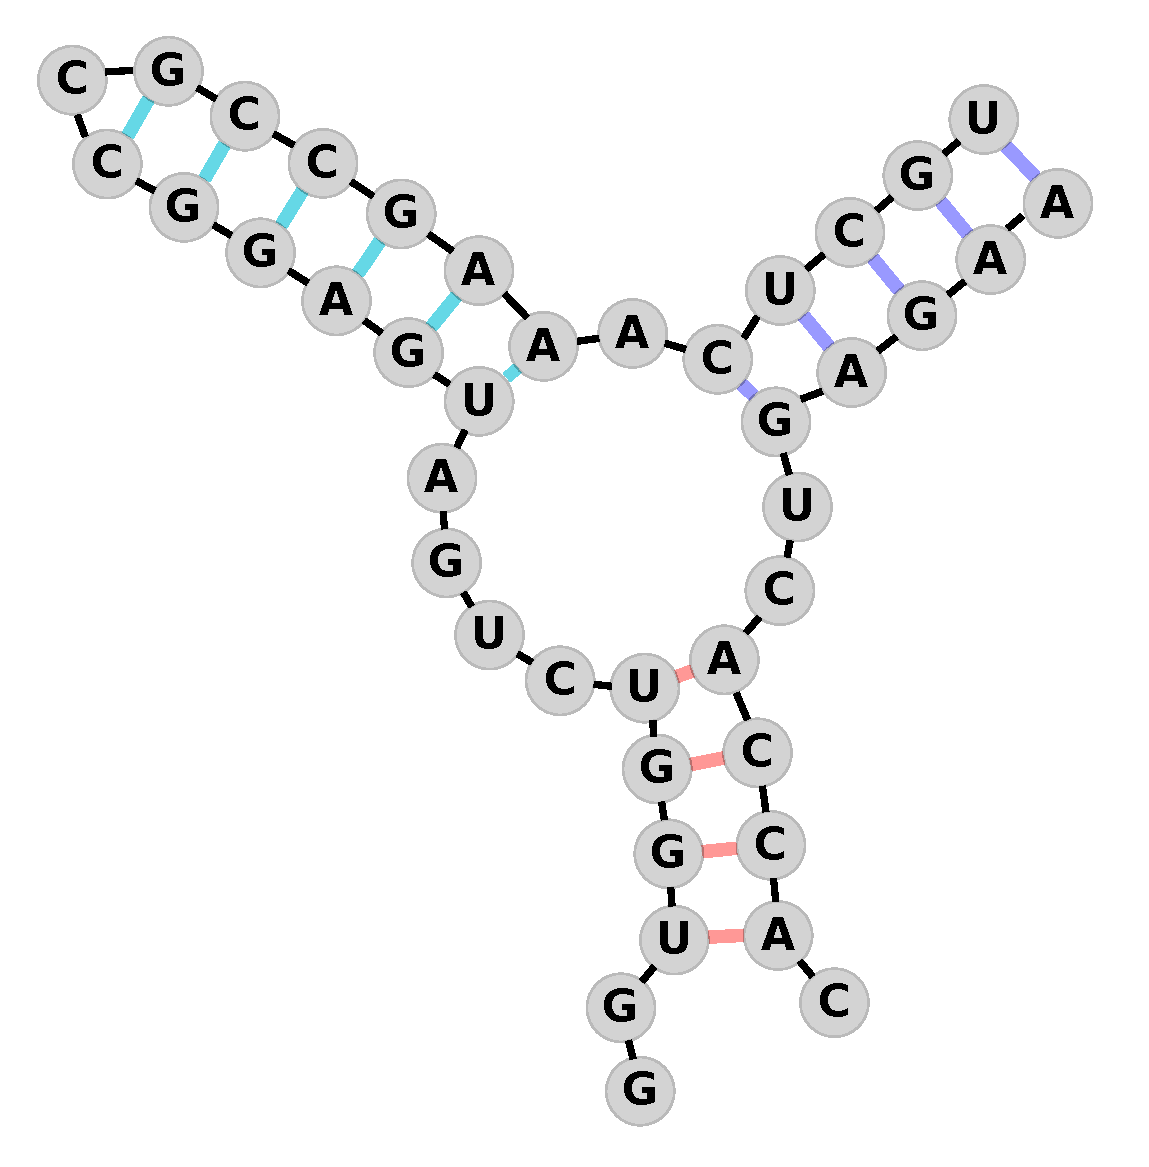
\includegraphics[width=\linewidth]{pics/struct.pdf}}
  \caption{Secondary structure visualization}
  \label{struc_a}
\end{subfigure}%
\begin{subfigure}{.33\textwidth}
  \centering
  \hbox{
\includegraphics[width=\linewidth]{pics/in.png}}
  \caption{Input image \\ for neural network}
  \label{struc_b}
\end{subfigure}
\begin{subfigure}{.33\textwidth}
  \centering
  \hbox{
\includegraphics[width=\linewidth]{pics/out.png}}
  \caption{Reference image \\ for neural network}
  \label{struc_c}
\end{subfigure}
\caption{Secondary structure representations}
\label{struc}
\end{figure}

\subsubsection{Parallel ResNet}
One of the popular architectures for complicated images processing tasks is a residual neural network based on adding skip connections between blocks of layers~\cite{he2016deep}. ResNets solve the problem of vanishing gradient and allow to effectively use deep convolutional networks.

In this work, we developed a new architecture that showed its applicability for secondary structure prediction task during experimental research. The idea is to combine $n$ identical residual networks that take the same input, go through independent sequences of layers and connect their $n$ outputs with weighted sum hanging it over to the final residual unit that directly generates output. This parallel residual architecture along with the scheme of a typical residual unit is presented in figure~\ref{nn}, where $k$ and $n$ can be selected based on empirical evidence. We believe that the advantage of this parallel technique is that these separate networks are able to find different types of features in data and some sort of voting system allows the whole model to decide for the particular pixel whether each network behaves correctly or not.

\begin{figure}[h]
\centering
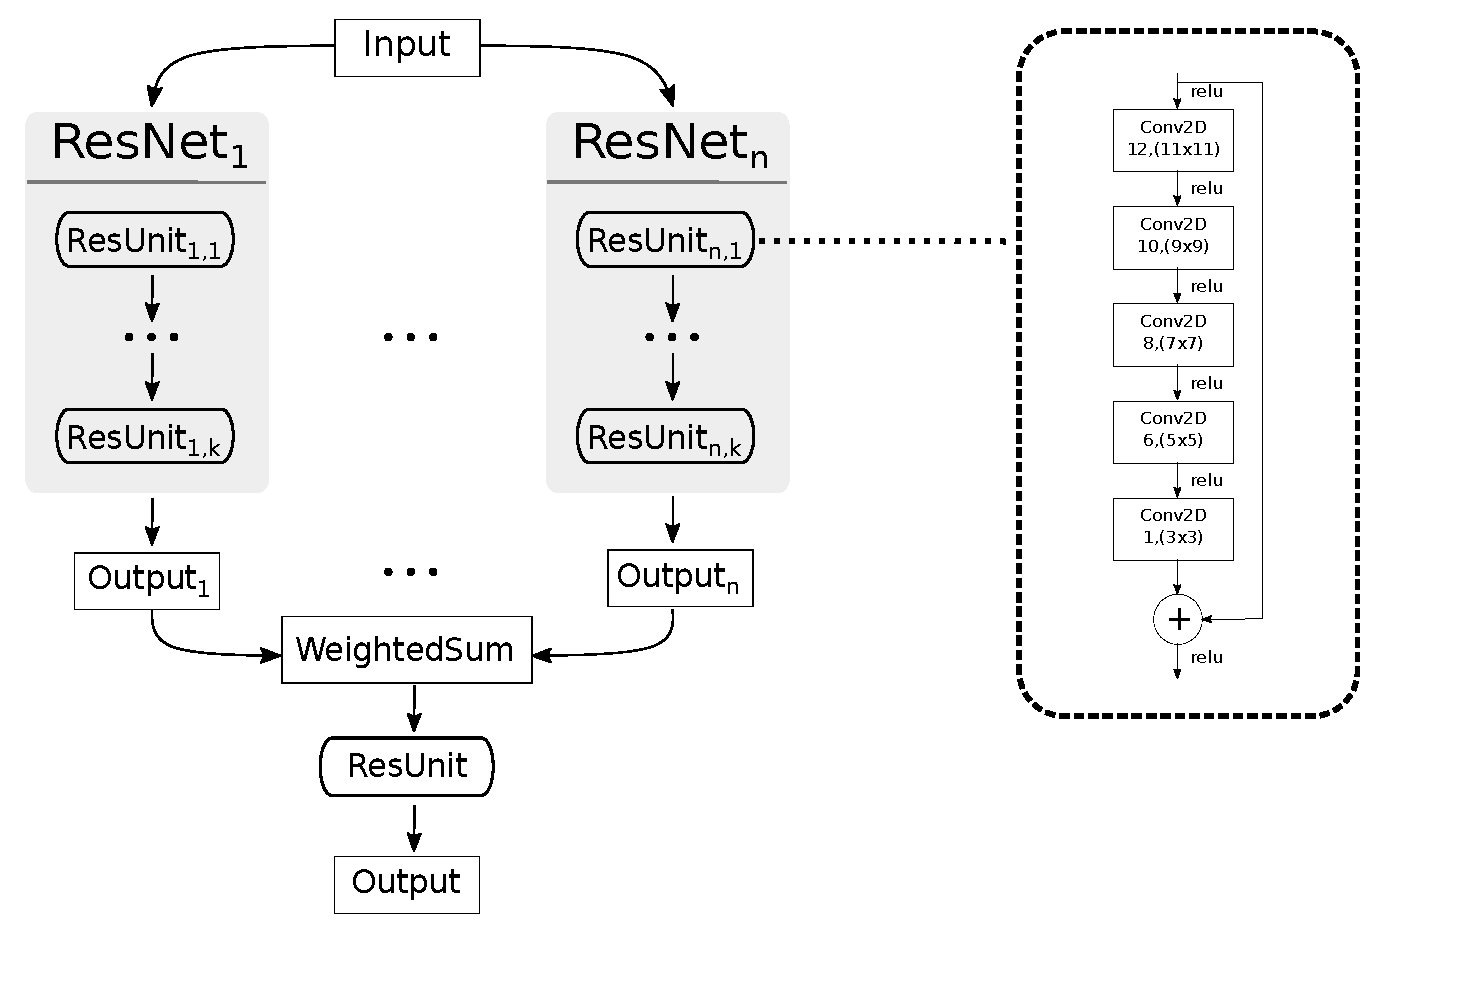
\includegraphics[width=\linewidth]{pics/nn.pdf}
\caption{Parallel ResNet architecture}
\label{nn}
\end{figure} 

\section{Experiments}
This section demonstrates the practical results of the proposed approach application. We introduce an easy-to-use implementation, specify some experimental details and describe currently available models. We compare our results with several popular tools and show the competitive power of our models.

\subsection{Tool}
The proposed approach was implemented as a Python console tool Genegram. Code, installation instructions, and documentation are available by link \linebreak \url{https://github.com/JetBrains-Research/Genegram}. This tool accepts a file with RNA sequences in fasta format and returns the connectivity tables (ct) for the corresponding secondary structures. We use an effective Python implementation of the parsing algorithm~\cite{Azimov:2018:CPQ:3210259.3210264} that shows high performance due to the GPGPU utilization and Keras~\cite{chollet2015keras} library with Tensorflow-GPU~\cite{tensorflow2015-whitepaper} framework for running the predictive model. Genegram tool allows to select different models and process sequences of lengths 1-200 containing only four canonical nucleotides.

\subsection{Setup}
The approach itself is quite flexible and Genegram tool provides a convenient environment for different experiments allowing to change both grammar and network. However, in the present work, we freeze grammar $G_0$ from figure~\ref{gram} and parallel ResNet architecture from figure~\ref{nn} with $k := 10$, $n := 4$. We consider only small RNAs (lengths from 1 to 200) due to the insufficient amount of longer sequences in biological databases and GPU storage limitations. Each sequence of $l$ nucleotides results in the image of size $l \times l$, therefore, images are grouped into batches by image size and cyclically duplicated until all batches have the same length. We use two data augmentation techniques on the training dataset: firstly, we mirror each image along the main diagonal (so that mirrored image represents the same sequence turned backwards), and secondly, we copy both regular and mirrored images twice. On this data, we run 10-fold cross-validation in order to choose the best train and validation split for each model.

The quality of the results is estimated by classical machine learning metrics calculated on the pixel-by-pixel difference between predicted and reference images. Further, we consider $TP$ (true positives, i.e. true white pixels), $FP$ (false positives, i.e. false white pixels), and $FN$ (false negatives, i.e. false black pixels) as numbers of right and wrong decisions among all contacts and calculate three following metrics for each image of some dataset. 

\begin{itemize} 
    \item $Precision = \displaystyle \frac{TP}{TP + FP}$ (proportion of correct contacts among all detected).
    \item $Recall = \displaystyle \frac{TP}{TP + FN}$ (proportion of detected contacts among all expected).
    \item $F1 = \displaystyle 2 * \frac{Precision * Recall}{Precision + Recall}$ (harmonic mean --- aggregation metrics).
\end{itemize}

The loss function is based on the idea of maximizing $F1$ score and that is to be achieved by minimizing the dataset mean $1 - F1$ through gradient descent. However, $F1$ is not differentiable as a function, so, we replace the sums of discrete integer values with a continuous sum of probabilities. Also, we charge our loss with two penalty coefficients responsible for huge dispersion between $Precision$ and $Recall$ for each image ($k1$) and the whole dataset ($k2$). Figure~\ref{loss} demonstrates the Python code for the currently used  $F1\_loss$ function that accepts two arguments: predicted image $y\_p$ and true image $y\_t$.

\begin{figure}[h]
\centering
\begin{lstlisting}[language=Python]
from keras import backend as K

def f1_loss(y_t, y_p):
    #normalize pixels values to [0, 1]
    y_t, y_p = K.minimum(y_t / 255, 1), K.minimum(y_p / 255, 1)
    #calculate differentiable versions of tw, fw and fb
    tw = K.sum(K.cast(y_t * y_p, 'float32'), axis=[1, 2, 3])
    fw = K.sum(K.cast((1 - y_t) * y_p, 'float32'), axis=[1, 2, 3])
    fb = K.sum(K.cast(y_t * (1 - y_p), 'float32'), axis=[1, 2, 3])
    #calculate precision and recall secure from zero division error
    prec = tw / (tw + fw + K.epsilon())
    rec = tw / (tw + fb + K.epsilon())
    #penalties for huge difference between precision and recall 
    #calculated for each image and whole dataset respectively
    k1 = 1 -  K.abs(prec- rec)
    k2 = 1 -  K.abs(K.mean(prec) - K.mean(rec))
    #calculate upgraded f1 score and return its mean value
    f1 = k1 * k2 * 2 * prec * rec / (prec + rec + K.epsilon()) 
    return 1 - K.mean(f1)
\end{lstlisting}
\caption{$F1\_loss$ function}
\label{loss}
\end{figure} 

For hyperparameters, we use Dropout after each residual unit to deal with overfitting, L2-regularization that also prevents overfitting and allows to search for complex data patterns, and Adagrad optimizer that automatically sets the learning rate and is known to be a powerful solution for sparse data processing.

For a comparative analysis of the results we selected six tools based on various concepts and algorithms. All of them demonstrate adequate speed and high accuracy, can handle pseudoknots and are easy to launch and use.

\begin{itemize}
    \item SPOT-RNA~\cite{singh2019rna} --- deep neural networks + transfer learning.
    \item Ipknot~\cite{sato2011ipknot} --- MEA + integer programming.
    \item Knotty~\cite{jabbari2018knotty} --- MFE + sparse dynamic programming.
    \item RNAstructure~\cite{bellaousov2013rnastructure} --- MFE + dynamic programming. 
    \item PknotsRG~\cite{reeder2007pknotsrg} --- MFE + Turner energy rules.
    \item HotKnots~\cite{ren2005hotknots} --- MFE + heuristic algorithm.
\end{itemize}

\subsection{Models}
In these conditions, we trained three identical networks on three different datasets and compared them with each other and with other tools by several criteria. All three models are available to use in the Genegram tool and the default model here is Genegram-main. Let us describe the specifics of each dataset, present the results of the best 10-fold cross-validation splits, and draw some conclusions.

\subsubsection{Genegram-main}
The first model was trained on data obtained from RNA STRAND database~\cite{andronescu2008rna} that is quite popular in different RNA analysis research due to its quality and usability. This database is an assembly of carefully curated and validated RNA sequences with secondary structures collected from different sources, and it contains only trustful structures obtained by reliable methods (laboratory or comparative). This database is supposed to provide the most representative sample of RNA secondary structures along with a guaranteed high quality of data which makes Genegram-main model trained on RNA STRAND the most general one for now, therefore, we set it as a default choice for our tool.

We selected 1091 sequences with lengths up to 200 and removed samples with gaps or inaccuracies in primary and secondary structures. The distribution of sequences lengths in the prepared dataset is demonstrated in figure~\ref{main_distr}. Neural network output images are grayscale and may contain multiple contacts, therefore, we applied binarization by threshold 0.6 with multiplets removal as postprocessing for this model and calculated the following metrics afterwards. Figure~\ref{main_f1} shows the estimation of Genegram-main and other six tools on validation set of size 109 by metrics $F1$. The shape of colored plots shows the density of $F1$ values, the red line represents its median result and the blue line corresponds to the mean one. It can be seen that Genegram-main has median $F1$ equal to 81 (as well as Knotty which is the second result after SPOT-RNA), and mean $F1$ equal to 70 that significantly exceeds the results of all competing tools except SPOT-RNA. The estimation on the same set by mean $Precision$ and $Recall$ metrics is presented in figure~\ref{main_pr}. Note that the binarization threshold allows us to slightly manipulate the balance between these two metrics and we choose it so that $F1$ mean value is the highest, even though it leads to a small excess of $Precision$ over $Recall$.

\begin{figure}[h]
\centering
    \subfloat[$F1$ distribution, mean, \\ and median on valid set]
        {\label{main_f1}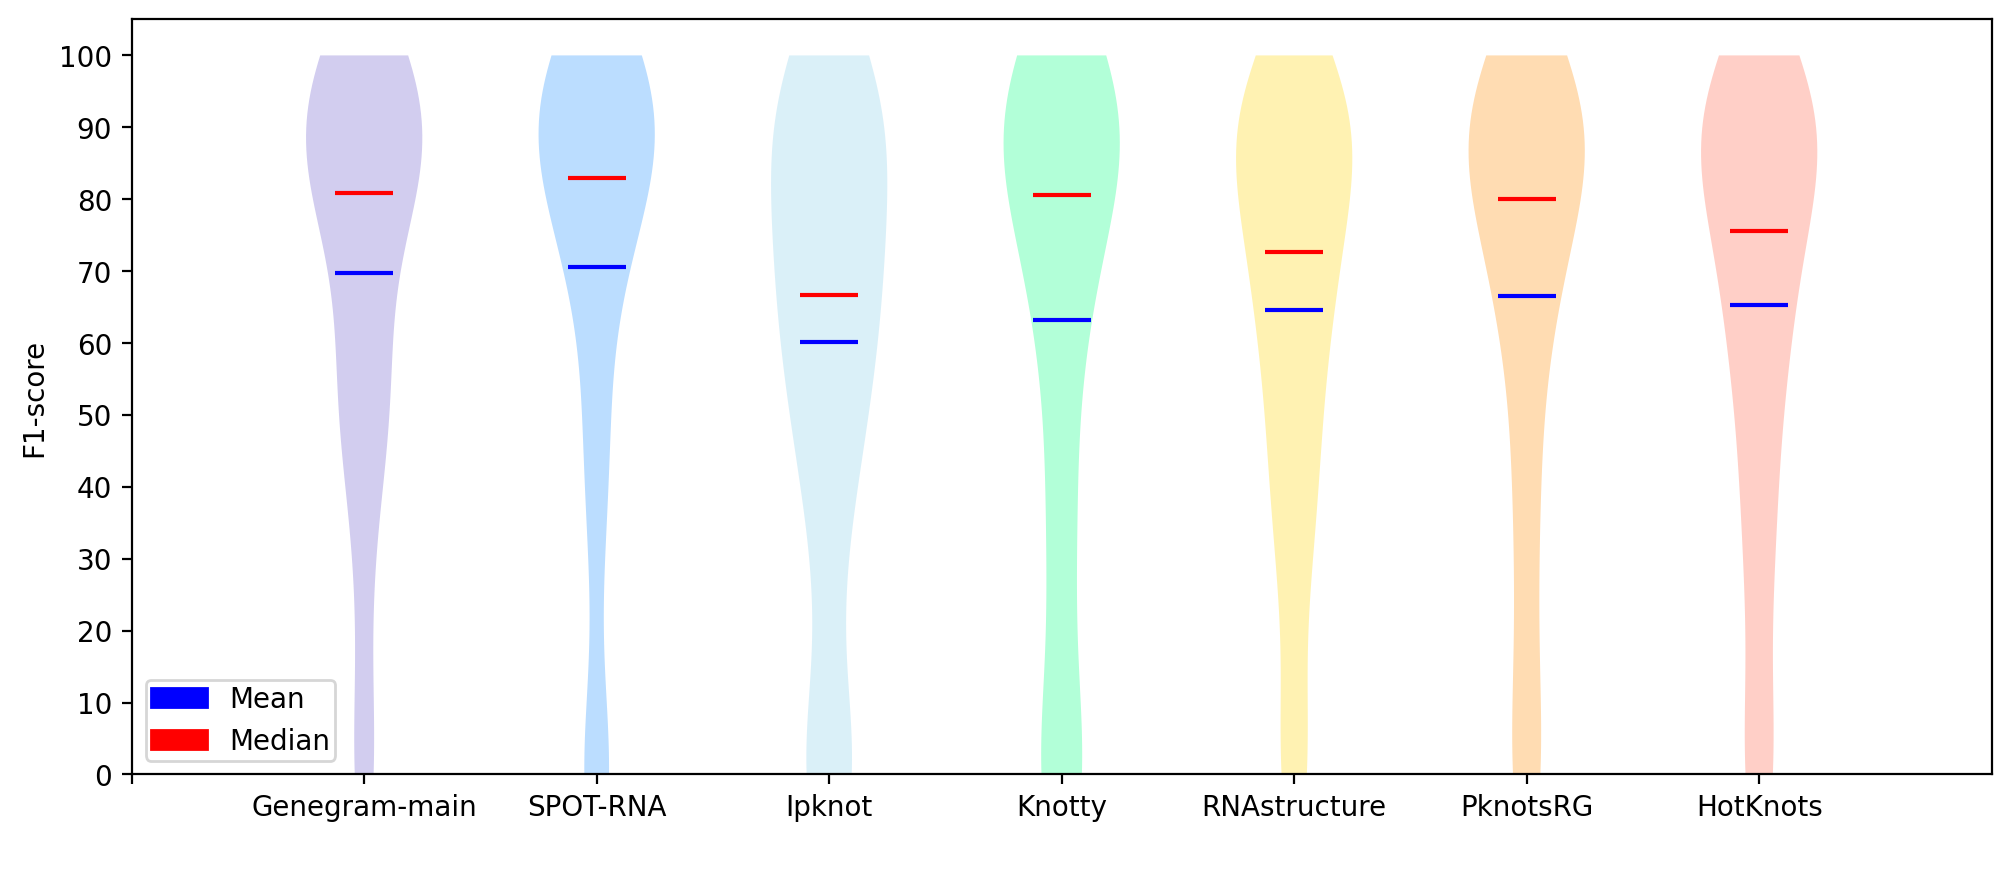
\includegraphics[width=.69\linewidth]{pics/plot_main_f1.png}}\hfill
    \subfloat[$Precision$ and $Recall$ mean on valid set]
        {\label{main_pr}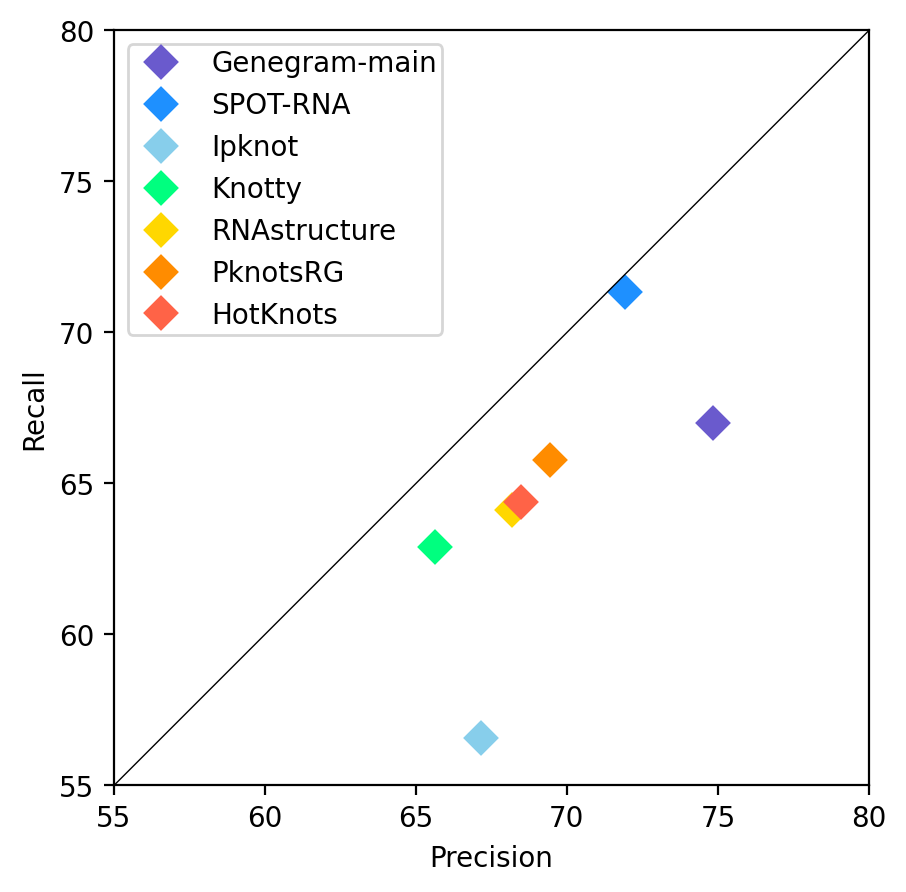
\includegraphics[width=.31\linewidth]{pics/plot_main_pr.png}}\par 
    \subfloat[Sequences lengths distribution on total set]
        {\label{main_distr}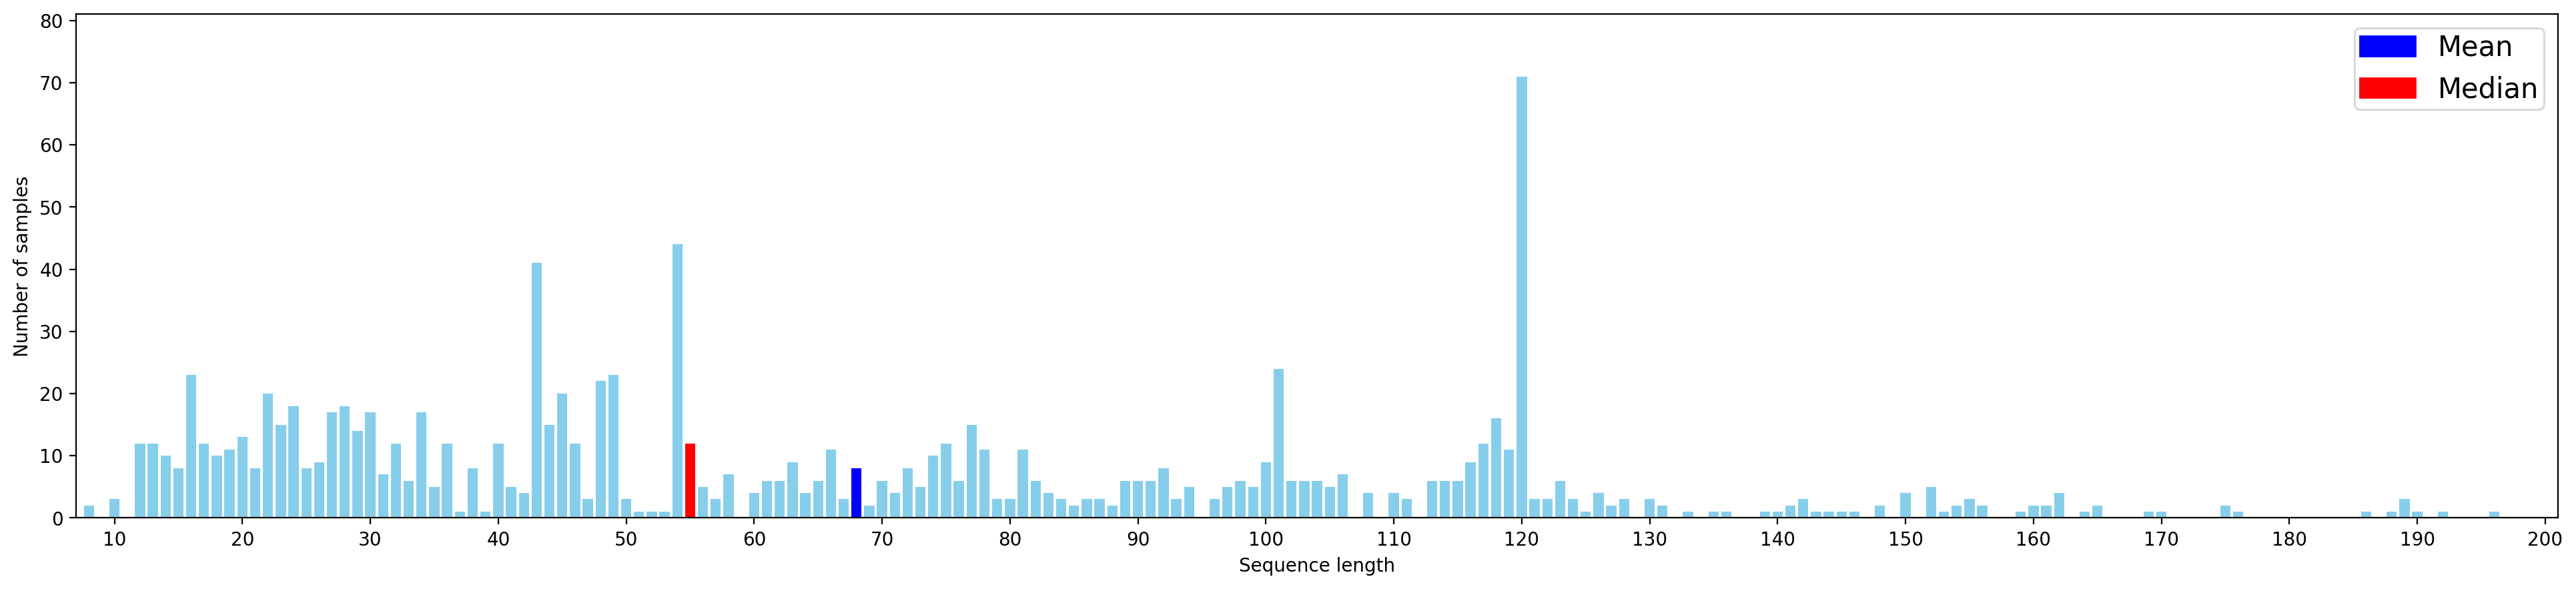
\includegraphics[width=\linewidth]{pics/plot_main_distr.png}}
\caption{Analysis of Genegram-main model compared with other tools }
\label{plots_main}
\end{figure}

All models were also estimated by several more specific functional criteria, such as pseudoknots prediction accuracy and sensitivity to different types of base pairs, so, table~\ref{table_main} demonstrates the results of these experiments. Considered validation set contained 11 pseudoknots and we calculated the number of correctly predicted contacts for each pseudoknot in each model output. The second column of table~\ref{table_main} shows the number of perfectly detected pseudoknots and the third column --- the number of ones that had up to 25\% extra or missing contacts. Clearly, pseudoknotted structures prediction is a non-trivial task for almost all models including Genegram-main. The other three columns of table~\ref{table_main} demonstrate how these tools handle different types of base pairs. Watson-Crick pairs are the most common and stable ones and it can be seen that all models have high enough canonical pairs prediction accuracy. Besides, it is known that wobble base pairs also have a biological role and regularly appear in real-world data, especially GU pair that has stability close to the Watson-Crick bonds. Our model slightly loses to other tools in GU pairs prediction, however, the great advantage of our approach is that it does not limit any types of pairs to be presented in neural network output (as well as SPOT-RNA that also uses neural networks), so, Genegram-main and SPOT-RNA are able to handle seven more wobble base pairs (AA, AC, AG, CC, CU, GG, UU), unlike other considered tools.

\begin{table}[h!]
\centering
\caption{Genegram-main and other models quality criteria measured on valid set}
\ra{1.4}
\begin{tabular}{@{}lccccccc@{}}\toprule
& \multicolumn{2}{c}{Pseudoknots} & \phantom{abc}& \multicolumn{3}{c}{Base pairs} \\
& No errors & 25\% errors  && Watson-Crick & GU & Others \\ \cmidrule{2-3} \cmidrule{5-7} 
Genegram-main  & 0 & 3 && 1067 & 68 & 53 \\
SPOT-RNA & 1 & 4 && 1190 & 134 & 39 \\
Ipknot & 0 & 1 && 939 & 92 & 0 \\
Knotty &1 & 3 && 1093 & 126 & 0 \\
RNAstructure & 1 & 1 && 1113 & 119 & 0 \\
PknotsRG & 1 & 5 && 1157 & 123 & 0 \\
HotKnots & 1 & 2 && 1113 & 112 & 0 \\
\bottomrule
Expected & 11 & 11 && 1650 & 185 & 135 \\
\bottomrule
\end{tabular}
\label{table_main}
\end{table}

\subsubsection{Genegram-pks}
Although the main model shows high results in general, it has poor pseudoknots prediction accuracy because RNA STRAND database contains only 86 sequences with pseudoknots and the neural network has not enough data to learn them, moreover, the amount of pseudoknots in the considered validation set is not enough to draw any conclusions. To improve this, we extended the previous dataset with sequences from Pseudobase~\cite{van2000pseudobase} database that is known to be a carefully built collection of pseudoknotted structures. Even though this database mostly contains not the whole sequences but only fragments with pseudoknots, we believe that the presence of such data in the training set may allow us to reach higher results in pseudoknots prediction.

We selected 1447 sequences having lengths up to 200 with no gaps or inaccuracies in primary and secondary structures and applied the same binarization by threshold 0.6 with multiplets removal as postprocessing. Note that both times we used 10-fold cross-validation on randomly shuffled data, so, Genegram-pks has separate from Genegram-main validation set, even though samples may intersect. Figure~\ref{pks_distr} shows the distribution of sequences lengths in total Genegram-pks dataset, figure~\ref{pks_f1} estimates all seven models on 145 validation sequences by $F1$ and figure~\ref{pks_pr} --- by $Precision$ and $Recall$ metrics. Genegram-pks is behind two tools by mean $F1$ value (70) and behind three tools by median (75) one, so, these results are quite competitive, however, Genegram-main was able to achieve the higher numbers.

\begin{figure}
\centering
    \subfloat[$F1$ distribution, mean, \\ and median on valid set]
        {\label{pks_f1}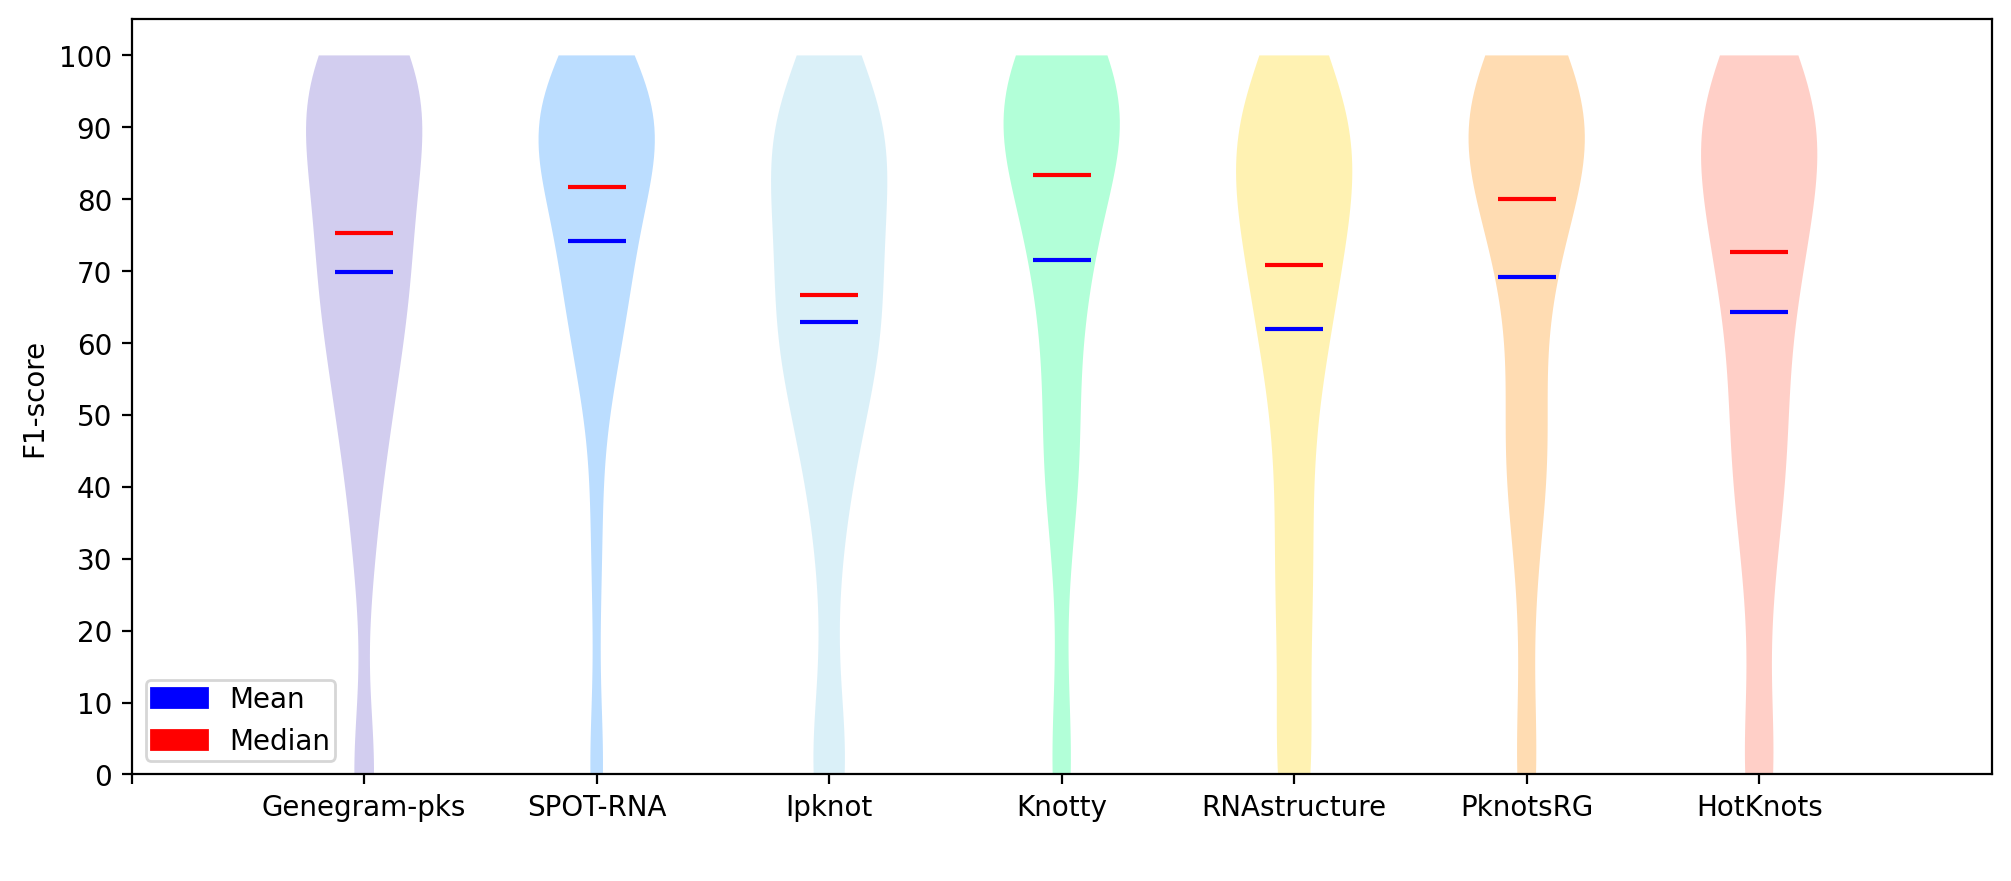
\includegraphics[width=.69\linewidth]{pics/plot_pks_f1.png}}\hfill
    \subfloat[$Precision$ and $Recall$ mean on valid set]
        {\label{pks_pr}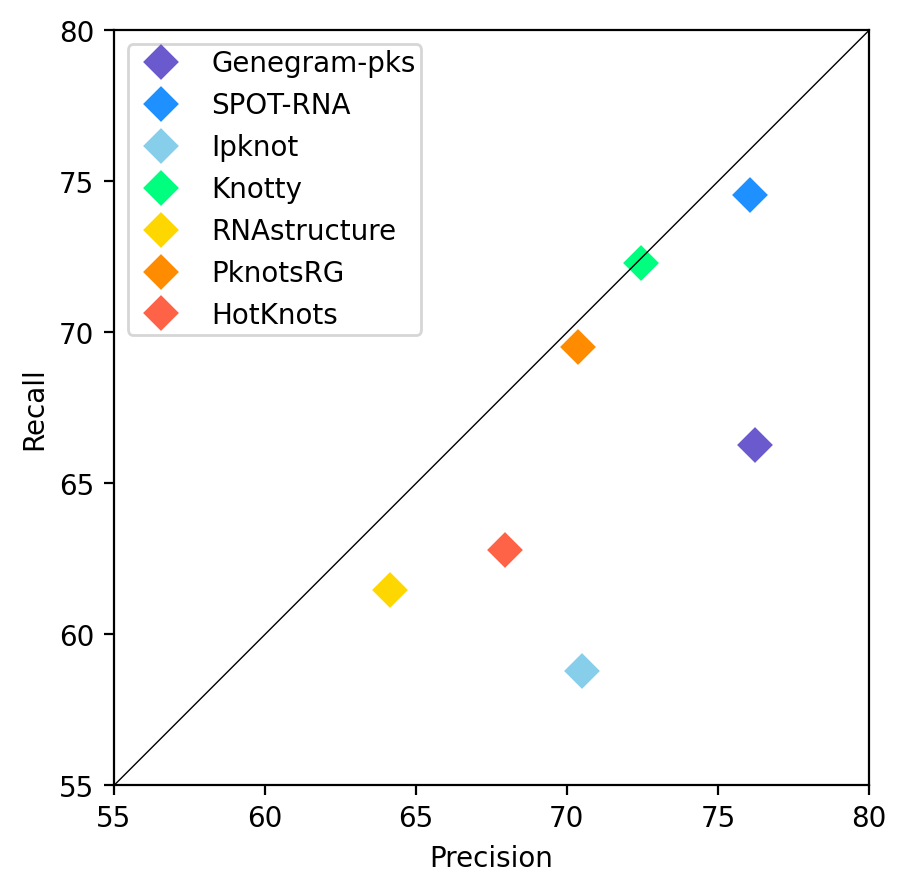
\includegraphics[width=.31\linewidth]{pics/plot_pks_pr.png}}\par 
    \subfloat[Sequences lengths distribution on total set]
        {\label{pks_distr}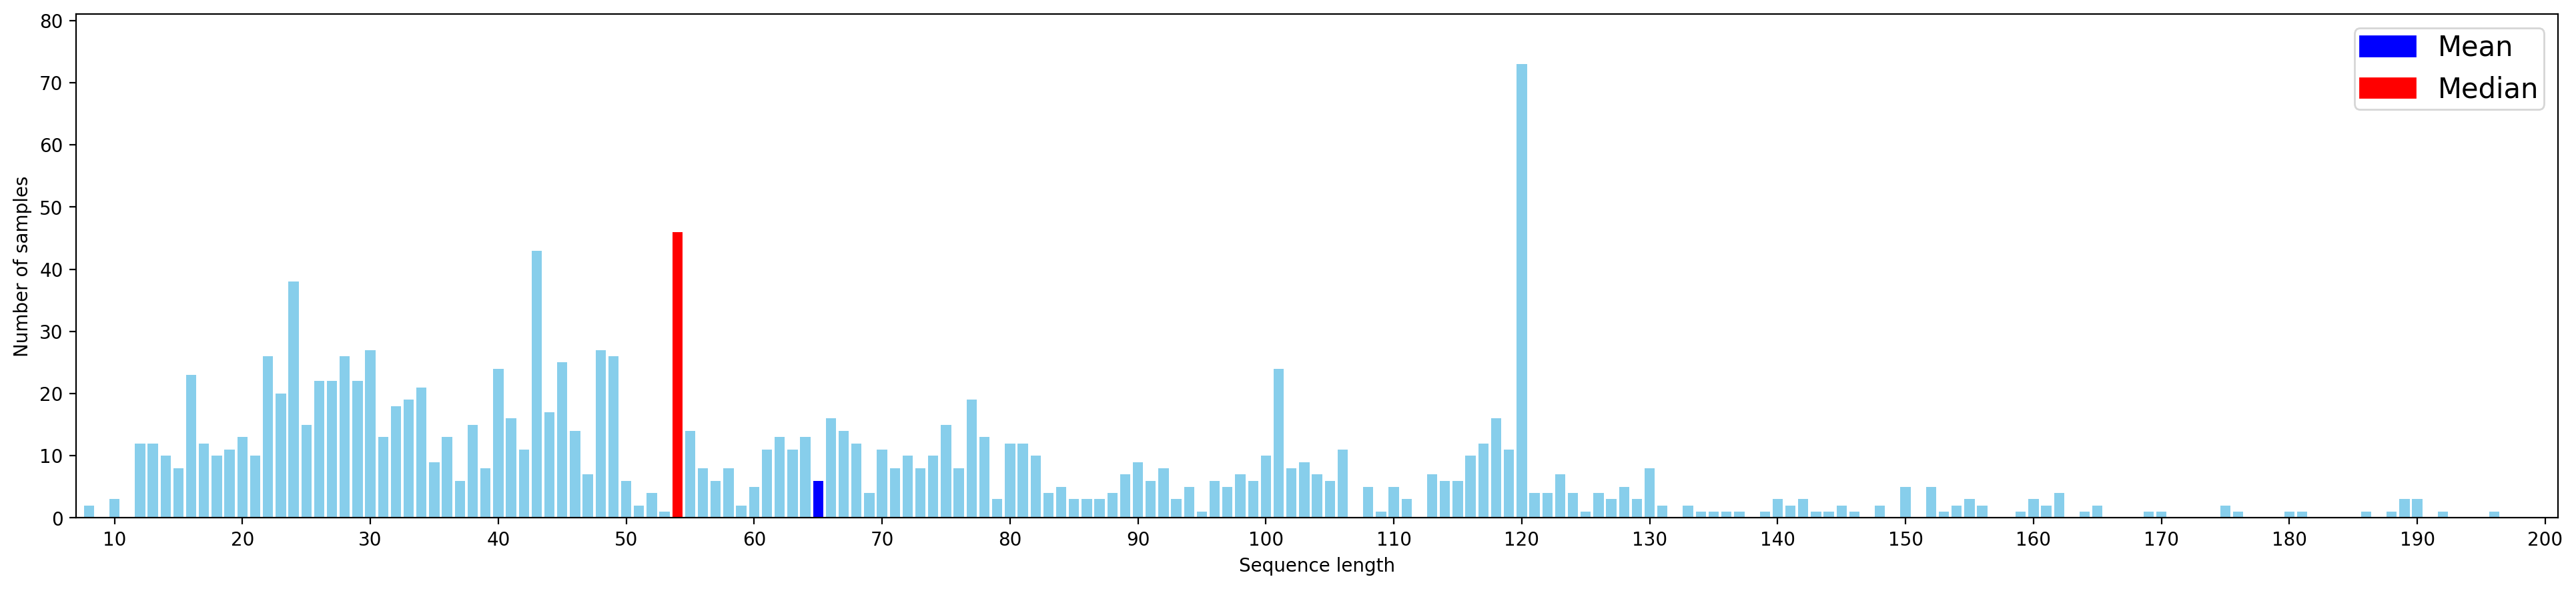
\includegraphics[width=\linewidth]{pics/plot_pks_distr.png}}
\caption{Analysis of Genegram-pks model compared with other tools }
\label{plots_pks}
\end{figure}

Similarly, we present the results of functional tests for this model and other tools in table~\ref{table_pks}. It can be seen that Watson-Crick pairs are predicted similarly to the main model, but wobble base pairs prediction accuracy decreased. However, the pseudoknotted structures processing was of particular interest in the context of Genegram-pks model and estimation by this criteria shows significant growth compared to the Genegram-main --- almost a quarter of all pseudoknots was detected perfectly, and about a half had small prediction errors. To sum up, this model generally losses to the main one, however, it shows very promising results in the aspect of pseudoknots detection being one of the best models for this problem.

\begin{table}
\centering
\caption{Genegram-pks and other models quality criteria measured on valid set}
\ra{1.4}
\begin{tabular}{@{}lccccccc@{}}\toprule
& \multicolumn{2}{c}{Pseudoknots} & \phantom{abc}& \multicolumn{3}{c}{Base pairs} \\
& No errors & 25\% errors  && Watson-Crick & GU & Others \\ \cmidrule{2-3} \cmidrule{5-7} 
Genegram-main  & 9 & 18 && 1628 & 61 & 47 \\
SPOT-RNA & 4 & 10 && 1893 & 173 & 71 \\
Ipknot & 2 & 5 && 1497 & 120 & 0 \\
Knotty & 11 & 20 && 1833 & 156 & 0 \\
RNAstructure & 3 & 7 && 1550 & 140 & 0 \\
PknotsRG & 11 & 20 && 1742 & 150 & 0 \\
HotKnots & 6 & 6 && 1621 & 143 & 0 \\
\bottomrule
Expected & 43 & 43 && 2407 & 258 & 156 \\
\bottomrule
\end{tabular}
\label{table_pks}
\end{table}

\subsubsection{Genegram-mps}
Another object that our approach allows to consider without any explicit definition is a multiplet that appears when base pair starts to form bonds with other bases or base pairs producing various topologies~\cite{bhattacharya2019going}. Multiplets are known to be functionally important, although, they are classified as tertiary structure features, so, secondary structure prediction tools are not usually able to handle them. In our terminology, multiplet would result in a reference image containing a set of white pixels where every two pixels have one equal coordinate, which makes multiplets processing possible in the terms of the considered approach.

For this experiment, we used data from PDB database~\cite{berman2000protein} that includes extracted from natural material RNA molecules with the corresponding crystallography results providing detailed structural information about secondary and tertiary interactions. This data tends to contain a lot of variability and complicated patterns, therefore, it creates more research possibilities but also makes it harder to learn. So, Genegram-mps is a network that was trained on data from the PDB database and for now, it is an experimental model that has possibilities in predicting more features, especially, multiplets. We selected 712 sequences with lengths up to 200 and kept samples with interactions with other molecules and up to 20\% unmodeled residues due to the insufficient amount of perfectly clean samples in this database. We used RNAView software~\cite{yang2003tools} to generate base pairs list from RNA crystallography files and extended $F1\_loss$ function with a penalty coefficient that considers the percentage of correctly predicted multiplets contacts in all images. Also, we applied a smaller binarization threshold of 0.45 for this model. Figure~\ref{mps_distr} demonstrates the distribution of sequences lengths in the whole dataset, figure~\ref{mps_f1} estimates all models on 71 validation sequences by $F1$ metrics and figure~\ref{mps_pr} --- by $Precision$ and $Recall$ metrics. Genegram-mps has a slightly lower $F1$ value than other tools, however, it shows the highest $Recall$ due to the fact that it is the only model that can predict multiplets. 

\begin{figure}
\centering
    \subfloat[$F1$ distribution, mean, \\ and median on valid set]
        {\label{mps_f1}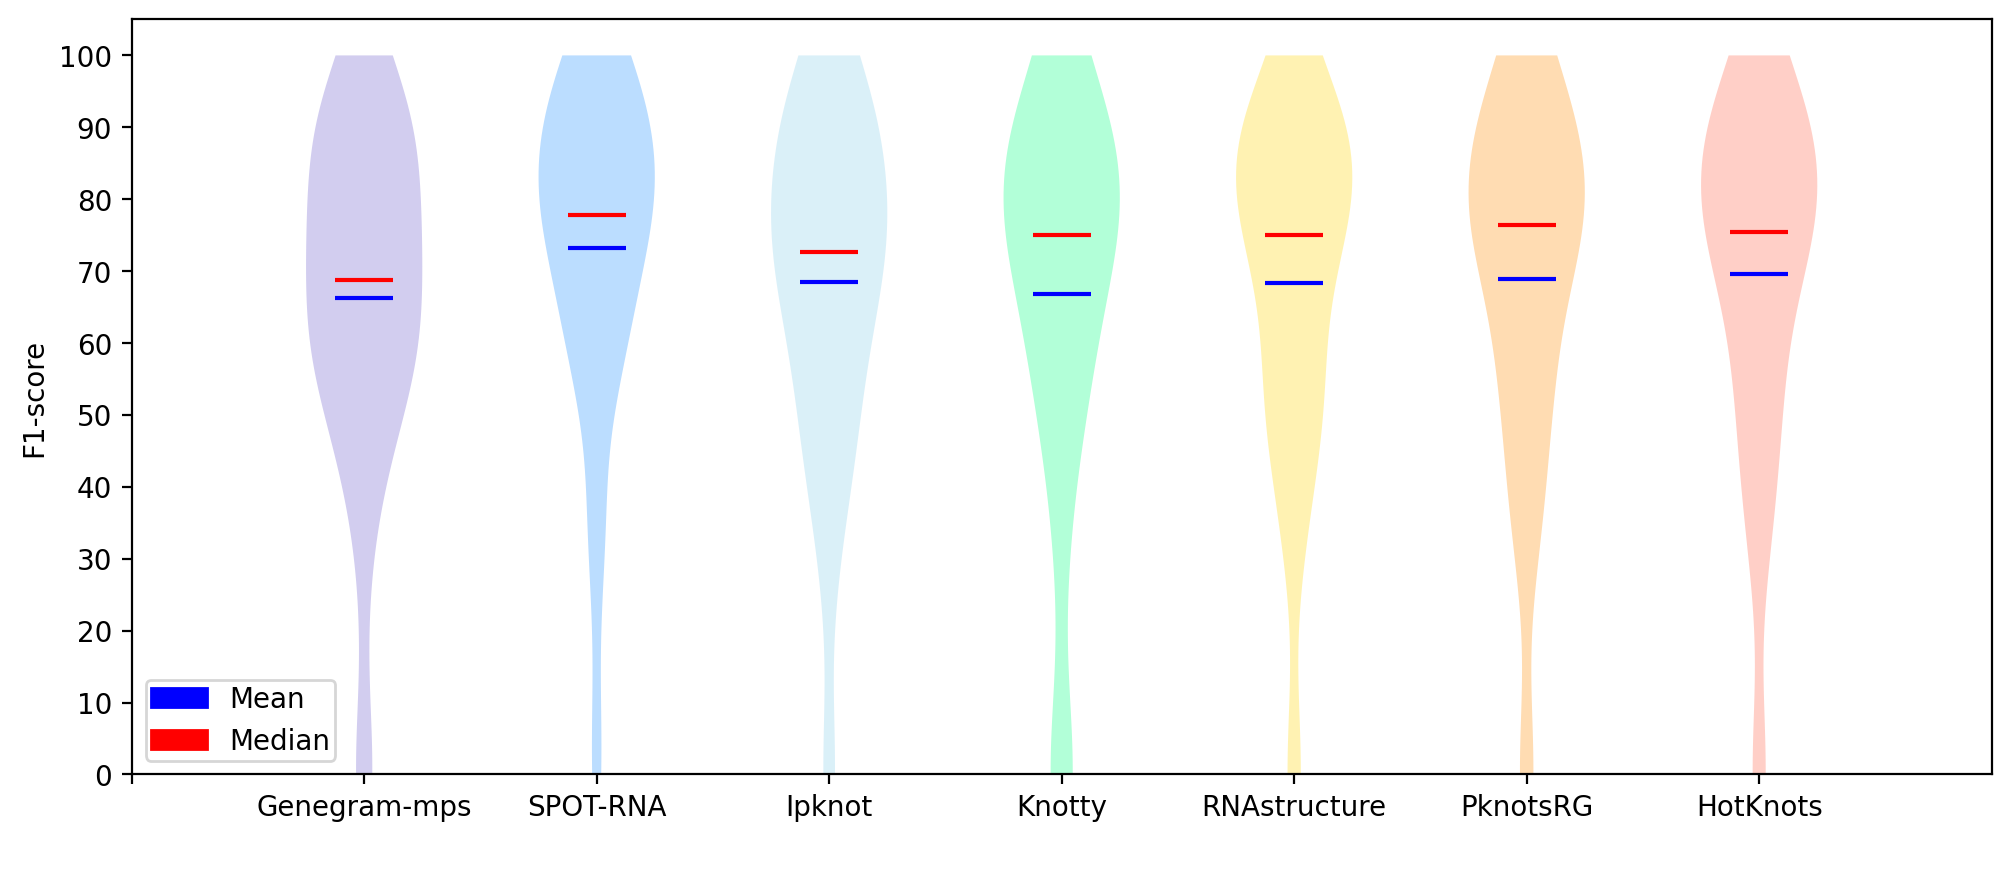
\includegraphics[width=.69\linewidth]{pics/plot_mps_f1.png}}\hfill
    \subfloat[$Precision$ and $Recall$ mean on valid set]
        {\label{mps_pr}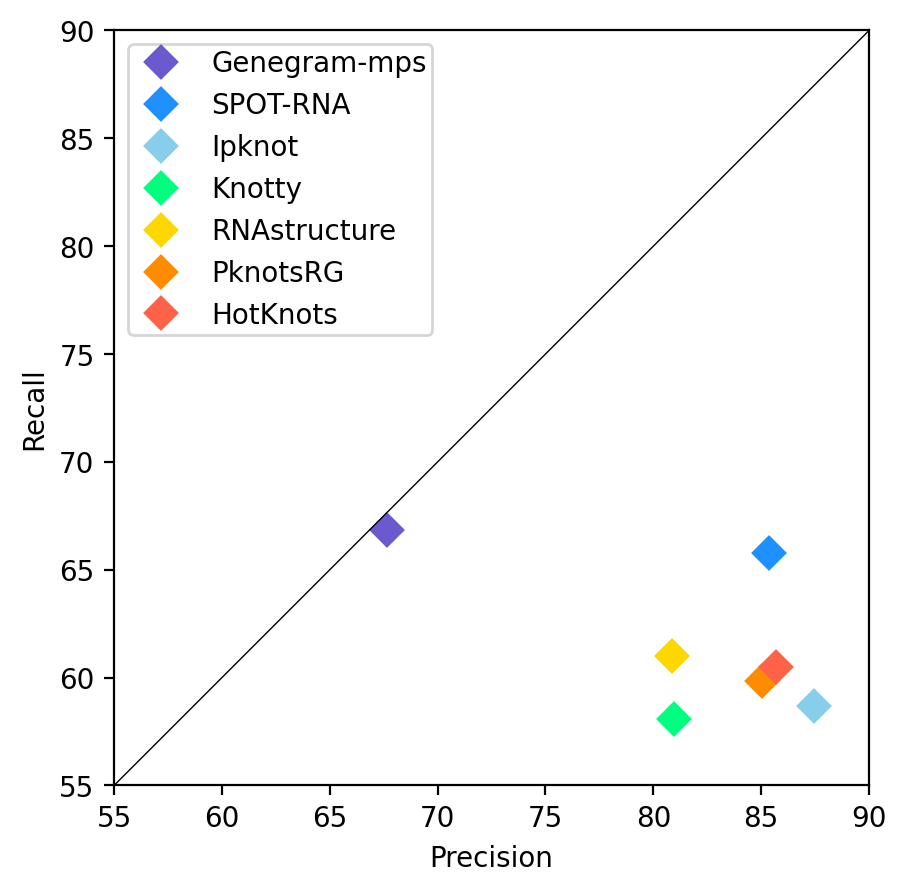
\includegraphics[width=.31\linewidth]{pics/plot_mps_pr.png}}\par 
    \subfloat[Sequences lengths distribution on total set]
        {\label{mps_distr}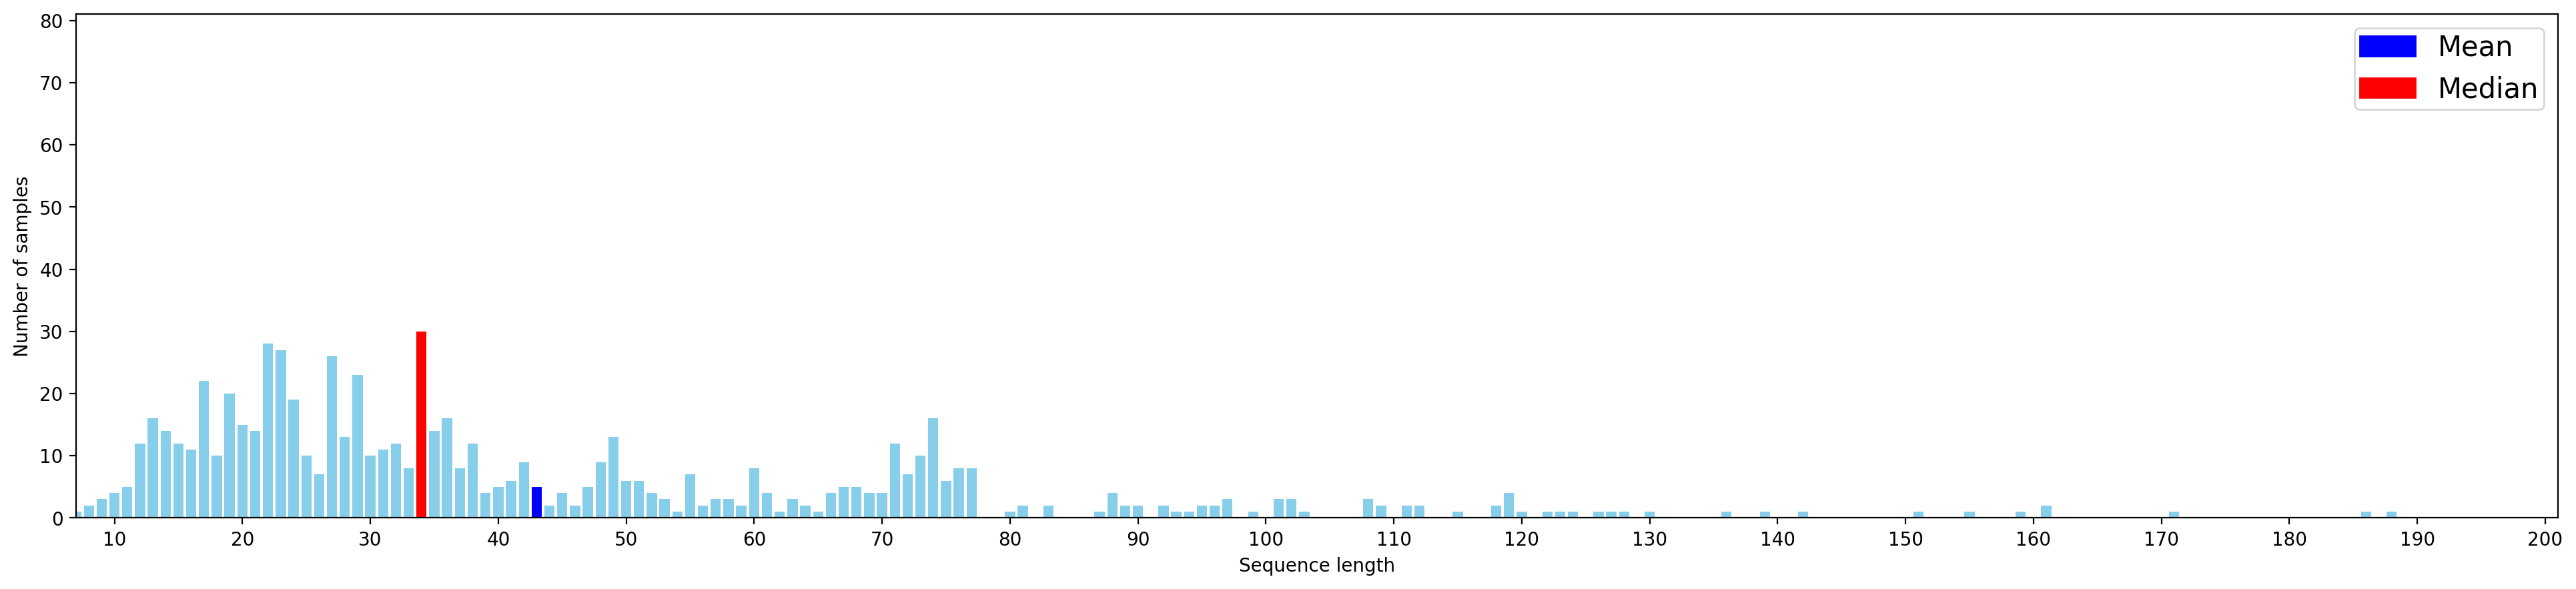
\includegraphics[width=\linewidth]{pics/plot_mps_distr.png}}
\caption{Analysis of Genegram-mps model compared with other tools }
\label{plots_pks}
\end{figure} 

As for functional tests, we similarly measured the prediction quality for three types of base pairs (table~\ref{table_mps}). Contacts belonging to multiplets are usually unstable, therefore, the ability of Genegram-mps model to predict multiplets resulted in high prediction accuracy for uncanonical base pairs. The definition of pseudoknot in the context of the multipletted structures is quite confusing, so, the estimation of pseudoknots was not run in this case. Instead of this, we provide the results of multiplets prediction. Note that there can be different ways of multiplets estimation and we choose two options for analysis: multiplets contacts (the amount of correct predictions among all contacts belonging to all multiplets in dataset) and multiplets pairs (the amount of correctly detected pairs $(i_1, j_1)$, $(i_2, j_2)$, where $i_1 = i_2$ or $i_1 = j_2$ or $j_1 = i_2$ or $j_1 = j_2$). The results of these tests are presented in the same table~\ref{table_mps}. It can be seen that all tools except Genegram are able to predict at most one contact of the multiplet pair and Genegram-mps model not only shows the highest contacts prediction score but also detects several paired interactions. However, the numbers are questionable so far, thus we introduce this model as a discussion about the possibilities of our approach rather than a final result.

\begin{table}[h!]
\centering
\caption{Genegram-mps and other models quality criteria measured on valid set}
\ra{1.4}
\begin{tabular}{@{}lccccccc@{}}\toprule
& \multicolumn{2}{c}{Multiplets} & \phantom{abc}& \multicolumn{3}{c}{Base pairs} \\
& Contacts & Pairs  && Watson-Crick & GU & Others \\ \cmidrule{2-3} \cmidrule{5-7} 
Genegram-mps  & 125 & 15 && 666 & 64 & 77 \\
SPOT-RNA & 101 & 0 && 680 & 64 & 44 \\
Ipknot & 67 & 0 && 630 & 56 & 0 \\
Knotty & 79 & 0 && 651 & 61 & 0 \\
RNAstructure & 73 & 0 && 643 & 62 & 0 \\
PknotsRG & 70 & 0 && 653 & 55 & 0 \\
HotKnots & 75 & 0 && 656 & 58 & 0 \\
\bottomrule
Expected & 448 & 395 && 863 & 132 & 316 \\
\bottomrule
\end{tabular}
\label{table_mps}
\end{table}

\subsubsection{Global tests}
In the previous sections we estimated three Genegram models separately on their validation sets and in this section, we provide some global tests for all the tools.

Due to the similar composition of training and validation sets for each model, the high results on validation make no reference to the general model quality, therefore, we downloaded several comparative and laboratory RNA secondary structure databases and evaluated Genegram models along with other tools on such data. These databases do not contain only purely selected structures, moreover, huge comparative databases usually aggregate a lot of homologous sequences with repetitive structural patterns, however, this experiment should check all models behavior on row data from various sources as opposed to the careful estimation on clean structures presented in the previous sections. We selected the following databases: CRW~\cite{cannone2002comparative}, Sprinzl~\cite{sprinzl1998compilation}, SRP~\cite{zwieb1992signal}, Rfam~\cite{griffiths2003rfam}, PDB~\cite{berman2000protein} (only single-chain samples without unmodelled bases) and Pseudobase~\cite{van2000pseudobase}. Note that most of these samples are completely new, however, some sequences or even databases could be previously used for some models training (e.g. Pseudobase was included in Genegram-pks training set). Table~\ref{table_all} represents the estimation of three Genegram models along with other tools by mean $F1$ score on all databases and the last column shows the mean $F1$ value among total samples. It can be seen that in most cases our models show adequate numbers regarding other tools, so, we can state that all neural networks generalize well on new datasets.

\begin{table}
\centering
\caption{All models estimation by $F1$ metrics on different databases}
\ra{1.4}
\begin{tabular}{@{}lcccccccc@{}}\toprule
& CRW & Sprinzl & SRP & Rfam & PDB & Pseudobase  & All data \\ \cmidrule{2-8} 
Genegram-main  & 69 & 73 & 59 & 43 & 74 & 42 & 69 \\
Genegram-pks  & 66 & 72 & 56 & 48 & 74 & 81 & 68 \\
Genegram-mps  &  &  &  &  &  &  &  \\
SPOT-RNA & 89 & 88 & 65 & 72 & 81 & 70 & 87 \\
Ipknot & 74 & 79 & 49 & 64 & 76 & 59 & 75 \\
Knotty & 74 & 75 & 63 & 63 & 79 & 76 & 74 \\
RNAstructure & 66 & 69 & 56 & 64 & 77 & 62 & 67 \\
PknotsRG & 62 & 61 & 65 & 66 & 79 & 77 & 62 \\
HotKnots & 61 & 60 & 66 & 66 & 78 & 61 & 61 \\
\bottomrule
Total samples & 11606 & 8777 & 360 & 1043 & 290 & 357 & 22433 \\
\bottomrule
\end{tabular}
\label{table_all}
\end{table}

Finally, we measured the time required for each tool to process fasta file with 100 RNA sequences and return secondary structure prediction for each sequence in its default output format. These tests were carried out on the workstation with the following characteristics: Ubuntu 20.04.2 LTS, Intel Core i5-10210U CPU 1.60GHz, NVIDIA GeForce MX250 GPU, and 7.5 GB RAM. We prepared two datasets by randomly selecting sequences from RNA STRAND database: the first set contained 100 sequences having lengths up to 100 and the second one --- 100 sequences with lengths up to 200. Table~\ref{table_time} shows the results of a performance experiment for such two fasta files. Genegram and SPOT-RNA were launched on GPU and the other tools have only CPU versions. It can be seen that the elapsed time spread among tools is quite big, moreover, several tools significantly lose in performance while processing longer sequences since various secondary structure prediction techniques may have completely different algorithmic complexity. However, Genegram shows an adequate performance due to the effective use of GPGPU in the parsing algorithm as well as in the neural network.

\begin{table}
\centering
\caption{Tools time performance on 100 sequences}
\ra{1.4}
\begin{tabular}{@{}lccc@{}}\toprule
& \multicolumn{2}{c}{\phantom{abc}  \phantom{abc}  \phantom{abc} Elapsed time, seconds}  \\
& Lengths 1-100 && Lengths 1-200  \\ \cmidrule{2-2} \cmidrule{4-4} 
Genegram & 28 && 39 \\
SPOT-RNA & 68 && 235 \\
Ipknot & 1 && 1 \\
Knotty & 283 && 3050 \\
RNAstructure & 10 && 15 \\
PknotsRG & 15 && 95 \\
HotKnots & 37 && 366 \\
\bottomrule
\end{tabular}
\label{table_time}
\end{table}

\section{Conclusion}
\section{Conclusion}

In this paper we present a library for sparse Boolean linear algebra which implements such basic operations as matrix-matrix multiplication and element-wise matrix-matrix addition in both Cuda and OpenCL.
Evaluation shows that our Boolean-specific implementations faster and require less memory than generic, not the Boolean optimized, operations from state-of-the-art libraries. 
Thus, the specialization of operations for this data type makes sense. 

The first direction of the future work is to integrate all parts (OpenCL and Cuda backends) into a single library and improve its documentation and prepare to publish.
Moreover, it is necessary to extend the library with other operations, including matrix-vector operations, masking, and so on.
As a result a Python package should be published.

Another important step is to evaluate the library on different algorithms and devices.
Namely, algorithms for RPQ and CFPQ should be implemented and evaluated on related data sets.
Also, it is necessary to evaluate OpenCL version on FPGA which may require additional technical effort and code changes.

Finally, we plan to discuss with GraphBLAS community possible ways to use our library as a backend for GraphBLAST or SuiteSparse in case of Boolean computations.
Moreover, it may be possible to use implemented algorithms as a foundation for generalization to arbitrary semirings.


%
\bibliography{main} 
\bibliographystyle{ieeetr}
\end{document}
